% VoxTell architecture (schematic), adapted from Rokuss et al., VoxTell, Fig. 2; layout after
% the author's sketch. Two versions of the stage the prompt decoder attends to:
%   paper (Ch. 3): keys/values = bottleneck F_5 (VoxTell Eq. 3; paper_notes/voxtell.md);
%   as used (Ch. 5): keys = encoder stage 4 + positional encoding, values = stage 4
%   (code/src/model/voxtell_model.py, transformer.py: pre-norm layer, cross-attention, feed-forward).
% Both: text encoder frozen, five fusion stages. Deep supervision (paper) is a training detail
% and not drawn; the figure shows the forward pass only.
% Switches (preamble.tex): \ifvoximpl draws the version as used instead of the paper's;
% \ifvoxannotate marks the strategies; \ifvoxpanel adds the prompt-decoder layer panel
% (a fact of the code as used, so Ch. 5 only).
% Ch. 3: impl, annotate, panel false. Ch. 5 (Fig. 5.1): all true.
%
% PLAN (rows, nodes, connections; all positions relative to X at the origin)
% Row 1 (image path): X -> enc -> fcol(f0..f5) ; brace over f0..f5 (right side) --skips--> dec.west ;
%   u1 -> u2 -> u3 -> u4 -> u5 (inside dec) ; u5.east -> Y.west (no loss node: the loss is computed
%   on the logits, not on the binary mask; removed 2026-10-29)
%   f<kv>.west -> left 2.5 mm -> below the column -> k1 -> PD.north   [keys, values]
%   (kv = 5, bottleneck, in the paper; kv = 4 as used)
% Row 2 (text path): P.north -> TE.south ; TE.east -> PD.west [q] ;
%   PD.east -> g1.west -> ... -> g5 (bus) ; g_i.north --dashed--> u_i.south (vertical)
% Row 3 (panel, main line ym; forward_pre: no self-attention): qin -> [mplus] -> j1 -> LN_A -> wq ;
%   memory: mem.south -> m-line (vertical) -> wv.west (values), wk.west (keys, + positional enc.) ;
%   [tokens v2.east -> m-line] ; wq/wk/wv.east -> att.west (three heights) ; (att.east |- wq) -> s1 ;
%   s1 -> j2 -> LN_B -> FFN -> s2 -> qnext ; residuals j1 -> s1.south, j2 -> s2.south (orthogonal,
%   one level below the cross-attention frame) ; [hpsi.south -> mplus.north]
% Annotations (Ch. 5): LoRA badges above wv / below wq ; KD frames around f4 and g1 ;
%   legend below the panel, two columns, each symbol a copy of the mark it explains.
\begin{tikzpicture}[
    font=\small, line width=0.5pt, >={Stealth[length=1.9mm, width=1.5mm]},
    every label/.style={font=\footnotesize},
    box/.style={draw, rounded corners=1.5pt, align=center, inner sep=2.5pt},
    lbl/.style={font=\footnotesize, align=center, inner sep=1pt},
    img/.style={inner sep=0pt},
    hidden/.style={inner sep=0pt, outer sep=0pt},
    feat/.style={draw, fill=voxred!25, minimum size=2.8mm, inner sep=0pt},
    sumc/.style={draw, circle, fill=white, inner sep=0pt, minimum size=3.6mm},
    guid/.style={draw, fill=voxblue!35, minimum width=2.2mm, minimum height=5mm, inner sep=0pt},
    bar/.style={draw, fill=voxgreen!45, minimum width=2mm, minimum height=5.5mm, inner sep=0pt},
    ln/.style={box, fill=voxyellow!60, minimum height=8mm, minimum width=6mm, inner sep=1pt},
    blk/.style={box, fill=voxyellow!35, minimum height=8mm},
    proj/.style={draw, fill=white, minimum width=6.5mm, minimum height=5mm, inner sep=1pt},
    lora/.style={draw=voxlora, fill=voxlora!12, text=voxlora!75!black, rounded corners=1pt, inner sep=1.5pt, font=\footnotesize},
    ptok/.style={draw=voxprompt, fill=voxprompt!30, minimum size=2.8mm, inner sep=0pt},
    kdframe/.style={draw=voxkd, densely dashed, line width=0.8pt, inner sep=0.9mm, rounded corners=1pt},
    dashedarrow/.style={->, densely dashed},
    res/.style={->, rounded corners=1.5pt},
  ]
\def\gap{5mm}
\ifvoximpl\def\kv{4}\else\def\kv{5}\fi   % encoder stage the prompt decoder attends to

% ===================== row 1: image path =====================
\node[img] (X) at (0,0) {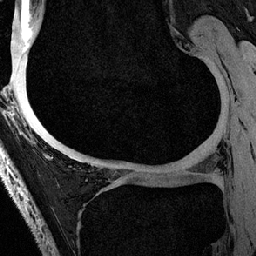
\includegraphics[width=16mm]{knee_patch.png}};
\node[lbl, below=1.5mm of X] (Xc) {$\mat{X}$\\$192^3$ patch};

\node[hidden, minimum width=20mm, minimum height=20mm, right=\gap of X] (enc) {};
\draw[fill=voxorange!25] (enc.north west) -- ([yshift=-5.5mm]enc.north east) -- ([yshift=5.5mm]enc.south east) -- (enc.south west) -- cycle;
\node[align=center] at ([xshift=-1.5mm]enc.center) {Image\\encoder};

\node[hidden, minimum width=2.8mm, minimum height=16.8mm, right=\gap of enc] (fcol) {};
\foreach \k in {0,...,5} { \node[feat] (f\k) at ([yshift=-1.4mm-2.8mm*\k]fcol.north) {}; }
\node[feat, line width=1.2pt] at (f\kv) {};
\draw[->] (enc.east) -- (fcol.west);

\coordinate (k1) at ([xshift=20mm]fcol.east);
\coordinate (kb) at ([yshift=-3mm]fcol.south);          % level of the keys/values route below the column

\node[hidden, minimum width=48mm, minimum height=20mm, right=24mm of fcol] (dec) {};
\draw[fill=voxorange!25] ([yshift=-5.5mm]dec.north west) -- (dec.north east) -- (dec.south east) -- ([yshift=5.5mm]dec.south west) -- cycle;
% skips: every encoder stage feeds the decoder stage of the same resolution (bottleneck = decoder input)
\draw[decorate, decoration={brace, amplitude=1.5mm}] ([xshift=1mm]fcol.north east) -- ([xshift=1mm]fcol.south east);
\coordinate (btip) at ([xshift=2.8mm]fcol.east);
\draw[dashedarrow] (btip) -- node[lbl, above, inner sep=1.5pt] {skips} (btip -| dec.west);
\node[sumc] (u1) at ([xshift=6.8mm]dec.west) {$\cdot$};
\foreach \i [evaluate=\i as \j using int(\i+1)] in {1,...,4} {
  \node[sumc, right=\gap of u\i] (u\j) {$\cdot$};
  \draw[->] (u\i.east) -- (u\j.west);
}
\node[lbl] at ([yshift=5mm]u3) {Decoder};

\node[img, right=6mm of dec] (Y) {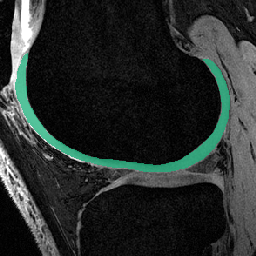
\includegraphics[width=16mm]{knee_patch_mask.png}};
\node[lbl, below=1.5mm of Y] {$\hat{\mat{Y}}$\\mask};
\draw[->] (u5.east) -- (Y.west);

% ===================== row 2: text path =====================
\coordinate (r2) at ([yshift=-30mm]X.center);
\node[box, fill=voxgreen!20, minimum width=24mm, minimum height=10mm, anchor=east] (PD) at ([xshift=4mm]k1 |- r2) {};
\foreach \k in {0,...,5} { \node[bar] (l\k) at ([xshift=-8mm+3.2mm*\k]PD.center) {}; }
\node[lbl, below=1.5mm of PD] {Prompt decoder\\($L_{\mathrm{dec}}$ layers)};
\coordinate (ka) at ([xshift=-2.5mm]f\kv.west);
\draw[->] (f\kv.west) -- (ka) |- (k1 |- kb) -- node[lbl, right, inner sep=2pt] {keys,\\values} (k1 |- PD.north);
\node[lbl, anchor=north west] at ([xshift=1mm, yshift=-1mm]ka |- kb) {\ifvoximpl stage 4\\($12^3$)\else bottleneck\\($6^3$)\fi};

\node[box, fill=voxblue!20, minimum height=10mm, left=7mm of PD] (TE) {Text encoder\\{\footnotesize Qwen3-Embedding-4B}};
\pic at ([xshift=-2.5mm, yshift=2.4mm]TE.north east) {lock};
\draw[->] (TE.east) -- node[above, inner sep=2pt] {$\vec{q}$} (PD.west);
\node[box, dashed, below=6mm of TE] (P) {``femoral cartilage''};
\node[lbl, below=1.5mm of P] {text prompt $p$};
\draw[->] (P.north) -- (TE.south);

\node[guid] (g1) at (u1 |- PD.east) {};
\draw (PD.east) -- (g1.west);
\foreach \i [evaluate=\i as \j using int(\i+1)] in {1,...,4} {
  \node[guid] (g\j) at (u\j |- PD.east) {};
  \draw (g\i.east) -- (g\j.west);
}
\foreach \i in {1,...,5} { \draw[dashedarrow] (g\i.north) -- (u\i.south); }
\node[lbl, right=2mm of g5, align=left] {guidance $\mat{E}_s$\\per decoder stage};

\ifvoxpanel
% ===================== row 3: one prompt-decoder layer =====================
% As built (normalize_before=True -> forward_pre, transformer.py:224-265): pre-norm
% cross-attention and feed-forward, each with a residual; the self-attention module of the
% layer is not used. Positional encoding is added to the keys only (value = memory).
\ifvoxannotate\coordinate (ym) at ([yshift=-80mm]r2);\else\coordinate (ym) at ([yshift=-76mm]r2);\fi
\node[anchor=west, inner sep=1pt] (qin) at ([xshift=3mm]X.west |- ym) {$\vec{q}$};
\ifvoxannotate
  \node[sumc, right=\gap of qin] (mplus) {$+$};
  \draw[->] (qin.east) -- (mplus.west);
  \coordinate (pre1) at (mplus.east);
\else
  \coordinate (pre1) at (qin.east);
\fi
\node[ln, right=6mm of pre1] (lnA) {LN};
\coordinate (j1) at ([xshift=3mm]pre1);
\draw[->] (pre1) -- (lnA.west);

% cross-attention with its projections; memory enters from above at W_v and W_k
\coordinate (mline) at ([xshift=4mm]lnA.east);
\node[proj, right=30mm of lnA] (wq) {$\mat{W}_q$};
\node[proj, above=5mm of wq] (wk) {$\mat{W}_k$};
\node[proj, above=5mm of wk] (wv) {$\mat{W}_v$};
\draw[->] (lnA.east) -- (wq.west);
\node[blk, minimum height=25mm, anchor=west] (att) at ([xshift=6mm]wq.east |- wk) {Attention};
\draw[->] (wq.east) -- (wq.east -| att.west);
\draw[->] (wk.east) -- (wk.east -| att.west);
\draw[->] (wv.east) -- (wv.east -| att.west);
\ifvoxannotate
  \node[lora, anchor=south west] (bv) at ([yshift=1mm]wv.north west) {$+\gamma_r\mat{B}\mat{A}$};
  \node[lora, anchor=north west] (bq) at ([yshift=-1mm]wq.south west) {$+\gamma_r\mat{B}\mat{A}$};
  \node[hidden, fit=(bv)(bq)] (cabox) {};
\else
  \node[hidden, fit=(wv)(wq)] (cabox) {};
\fi
\node[lbl, anchor=south east, font=\small] (catitle) at ([yshift=1.5mm]att.east |- cabox.north) {Cross-attention};
\begin{scope}[on background layer]
  \node[draw, rounded corners=2pt, fill=voxyellow!25, inner sep=2.5mm, fit=(cabox)(att)(catitle)] (ca) {};
\end{scope}

% keys and values: encoder stage-4 features; positional encoding on the keys only
\node[lbl, anchor=south west] (mem) at ([xshift=-1mm, yshift=8mm]mline |- ca.north) {stage-4 image features};
\draw (mem.south west -| mline) -- (mline |- wv);
\draw[->] (mline |- wv) -- (wv.west);
\draw[->] (mline |- wv) -- (mline |- wk) -- (wk.west);
\node[lbl, anchor=south west, align=left, inner sep=1.5pt] at ([xshift=2mm, yshift=0.5mm]mline |- wk) {$+$ positional\\encoding};

% feed-forward sub-layer
\node[sumc, anchor=west] (s1) at ([xshift=6mm]att.east |- wq) {$+$};
\draw[->] (att.east |- wq) -- (s1.west);
\node[ln, right=6mm of s1] (lnB) {LN};
\node[blk, right=\gap of lnB] (ff) {FFN};
\node[sumc, right=\gap of ff] (s2) {$+$};
\node[right=\gap of s2, inner sep=1pt] (qnext) {$\vec{q}'$};
\coordinate (j2) at ([xshift=3mm]s1.east);
\draw[->] (s1.east) -- (lnB.west);
\draw[->] (lnB.east) -- (ff.west);
\draw[->] (ff.east) -- (s2.west);
\draw[->] (s2.east) -- (qnext.west);

% residual connections, one level below the cross-attention frame
\coordinate (rl) at ([yshift=-4mm]ca.south);
\foreach \j/\s in {j1/s1, j2/s2} { \draw[res] (\j) |- (rl -| \s) -- (\s.south); }

\ifvoxannotate
  % learned prompt tokens appended to keys/values (layers l <= L_p)
  \node[ptok, anchor=west] (v1) at ([xshift=3mm, yshift=3.5mm]mline |- ca.north) {};
  \node[ptok, right=0.4mm of v1] (v2) {};
  \node[lbl, right=1mm of v2, text=voxprompt!80!black] {learned tokens $\mat{V}_l$ appended};
  \draw[->, voxprompt] (v1.west) -- (v1.west -| mline);
  % meta-net: offset of the text query (layers l <= L_p)
  \node[box, draw=voxmeta, fill=voxmeta!15, above=6mm of mplus] (hpsi) {$h_\psi$};
  \draw[->, voxmeta] (hpsi.south) -- node[lbl, right, text=voxmeta!80!black] {$\Delta\vec{q}$} (mplus.north);
  % (inputs of h_psi -- q and the mean of the keys -- are stated in the caption)
  % distillation: stage-4 features and stage-4 guidance
  \node[kdframe, fit=(f4)] {};
  \node[kdframe, fit=(g1)] {};
\fi

% panel frame with title
\node[anchor=south west, inner sep=1pt] (ptitle) at ([yshift=2mm]qin.west |- mem.north) {Prompt-decoder layer $l = 1, \dots, L_{\mathrm{dec}}$};
\coordinate (pright) at ([xshift=-2.5mm]Y.east |- ym);   % panel ends flush with row 1
\begin{pgfonlayer}{panel}
  \node[draw, rounded corners=3pt, fill=voxgreen!8, inner sep=2.5mm, fit=(ptitle)(qin)(qnext)(ca)(mem)(rl)(pright)] (panel) {};
\end{pgfonlayer}

\ifvoxannotate
  % legend: each symbol repeats the mark used in the figure
  \node[lora, minimum width=6mm, minimum height=3.2mm, anchor=north west] (lg1) at ([xshift=1mm, yshift=-2.5mm]panel.south west) {};
  \node[lbl, right=1.5mm of lg1, anchor=west] {LoRA: $\mat{W}_q$, $\mat{W}_v$ in all layers};
  \node[kdframe, inner sep=0pt, minimum width=6mm, minimum height=3.2mm, below=2.2mm of lg1] (lg2) {};
  \node[lbl, right=1.5mm of lg2, anchor=west] {distillation: stage-4 features, guidance $\mat{E}_4$};
  \node[ptok, anchor=north west] (lg3a) at ([xshift=2mm, yshift=-2.7mm]panel.south) {};
  \node[ptok, right=0.4mm of lg3a] (lg3) {};
  \node[lbl, right=1.5mm of lg3, anchor=west] {prompt tuning: tokens $\mat{V}_l$, layers $l \le L_p$};
  \node[box, draw=voxmeta, fill=voxmeta!15, inner sep=0pt, minimum width=6mm, minimum height=3.2mm, anchor=west] (lg4) at (lg3a.west |- lg2) {};
  \node[lbl, right=1.5mm of lg4, anchor=west] {prompt tuning: meta-net $h_\psi$, layers $l \le L_p$};
\fi
\fi % voxpanel
\end{tikzpicture}
